\documentclass{article}

\usepackage{tikz}

\begin{document}
  \begin{figure}[h]
    \begin{center}
      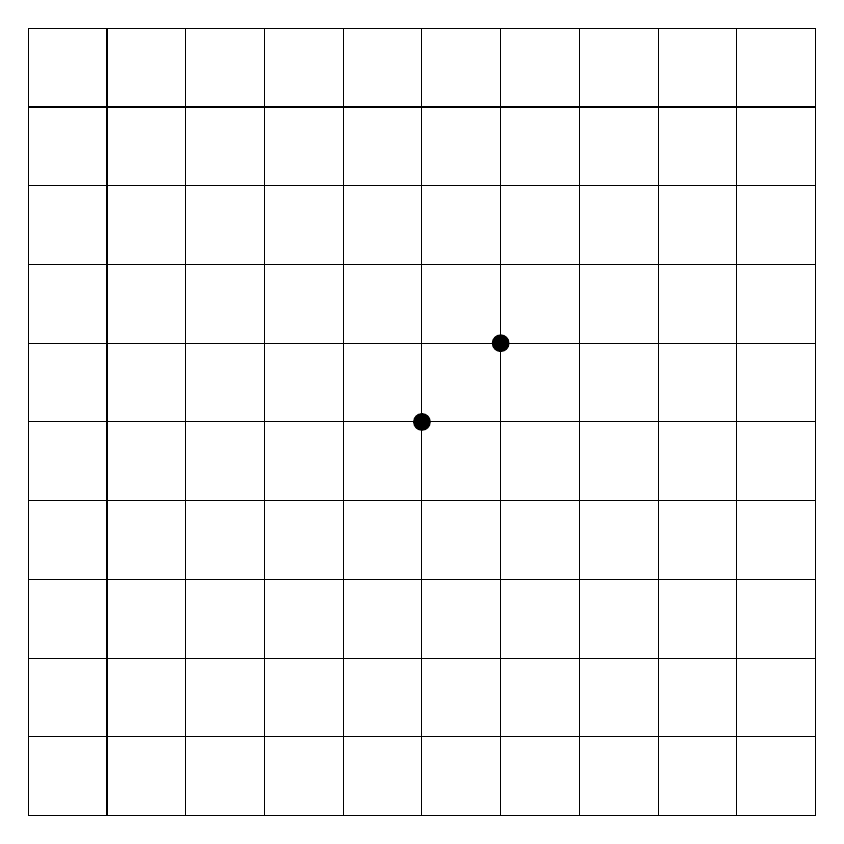
\begin{tikzpicture}
        \draw(-5,-5) grid (5,5);
        \filldraw[black](0,0)circle[radius=3pt];
        \filldraw[black](1,1)circle[radius=3pt];
      \end{tikzpicture}
      \caption{\label{my_grid}A grid with two points!}
    \end{center}
  \end{figure}
\end{document}